
%% bare_conf.tex
%% V1.4b
%% 2015/08/26
%% by Michael Shell
%% See:
%% http://www.michaelshell.org/
%% for current contact information.
%%
%% This is a skeleton file demonstrating the use of IEEEtran.cls
%% (requires IEEEtran.cls version 1.8b or later) with an IEEE
%% conference paper.
%%
%% Support sites:
%% http://www.michaelshell.org/tex/ieeetran/
%% http://www.ctan.org/pkg/ieeetran
%% and
%% http://www.ieee.org/

%%*************************************************************************
%% Legal Notice:
%% This code is offered as-is without any warranty either expressed or
%% implied; without even the implied warranty of MERCHANTABILITY or
%% FITNESS FOR A PARTICULAR PURPOSE! 
%% User assumes all risk.
%% In no event shall the IEEE or any contributor to this code be liable for
%% any damages or losses, including, but not limited to, incidental,
%% consequential, or any other damages, resulting from the use or misuse
%% of any information contained here.
%%
%% All comments are the opinions of their respective authors and are not
%% necessarily endorsed by the IEEE.
%%
%% This work is distributed under the LaTeX Project Public License (LPPL)
%% ( http://www.latex-project.org/ ) version 1.3, and may be freely used,
%% distributed and modified. A copy of the LPPL, version 1.3, is included
%% in the base LaTeX documentation of all distributions of LaTeX released
%% 2003/12/01 or later.
%% Retain all contribution notices and credits.
%% ** Modified files should be clearly indicated as such, including  **
%% ** renaming them and changing author support contact information. **
%%*************************************************************************


% *** Authors should verify (and, if needed, correct) their LaTeX system  ***
% *** with the testflow diagnostic prior to trusting their LaTeX platform ***
% *** with production work. The IEEE's font choices and paper sizes can   ***
% *** trigger bugs that do not appear when using other class files.       ***                          ***
% The testflow support page is at:
% http://www.michaelshell.org/tex/testflow/



\documentclass[conference]{IEEEtran}
% Some Computer Society conferences also require the compsoc mode option,
% but others use the standard conference format.
%
% If IEEEtran.cls has not been installed into the LaTeX system files,
% manually specify the path to it like:
% \documentclass[conference]{../sty/IEEEtran}





% Some very useful LaTeX packages include:
% (uncomment the ones you want to load)


% *** MISC UTILITY PACKAGES ***
%
%\usepackage{ifpdf}
% Heiko Oberdiek's ifpdf.sty is very useful if you need conditional
% compilation based on whether the output is pdf or dvi.
% usage:
% \ifpdf
%   % pdf code
% \else
%   % dvi code
% \fi
% The latest version of ifpdf.sty can be obtained from:
% http://www.ctan.org/pkg/ifpdf
% Also, note that IEEEtran.cls V1.7 and later provides a builtin
% \ifCLASSINFOpdf conditional that works the same way.
% When switching from latex to pdflatex and vice-versa, the compiler may
% have to be run twice to clear warning/error messages.






% *** CITATION PACKAGES ***
%
\usepackage{cite}
% cite.sty was written by Donald Arseneau
% V1.6 and later of IEEEtran pre-defines the format of the cite.sty package
% \cite{} output to follow that of the IEEE. Loading the cite package will
% result in citation numbers being automatically sorted and properly
% "compressed/ranged". e.g., [1], [9], [2], [7], [5], [6] without using
% cite.sty will become [1], [2], [5]--[7], [9] using cite.sty. cite.sty's
% \cite will automatically add leading space, if needed. Use cite.sty's
% noadjust option (cite.sty V3.8 and later) if you want to turn this off
% such as if a citation ever needs to be enclosed in parenthesis.
% cite.sty is already installed on most LaTeX systems. Be sure and use
% version 5.0 (2009-03-20) and later if using hyperref.sty.
% The latest version can be obtained at:
% http://www.ctan.org/pkg/cite
% The documentation is contained in the cite.sty file itself.


\usepackage{graphicx}



% *** GRAPHICS RELATED PACKAGES ***
%
\ifCLASSINFOpdf
  % \usepackage[pdftex]{graphicx}
  % declare the path(s) where your graphic files are
  % \graphicspath{{../pdf/}{../jpeg/}}
  % and their extensions so you won't have to specify these with
  % every instance of \includegraphics
  % \DeclareGraphicsExtensions{.pdf,.jpeg,.png}
\else
  % or other class option (dvipsone, dvipdf, if not using dvips). graphicx
  % will default to the driver specified in the system graphics.cfg if no
  % driver is specified.
  % \usepackage[dvips]{graphicx}
  % declare the path(s) where your graphic files are
  % \graphicspath{{../eps/}}
  % and their extensions so you won't have to specify these with
  % every instance of \includegraphics
  % \DeclareGraphicsExtensions{.eps}
\fi
% graphicx was written by David Carlisle and Sebastian Rahtz. It is
% required if you want graphics, photos, etc. graphicx.sty is already
% installed on most LaTeX systems. The latest version and documentation
% can be obtained at: 
% http://www.ctan.org/pkg/graphicx
% Another good source of documentation is "Using Imported Graphics in
% LaTeX2e" by Keith Reckdahl which can be found at:
% http://www.ctan.org/pkg/epslatex
%
% latex, and pdflatex in dvi mode, support graphics in encapsulated
% postscript (.eps) format. pdflatex in pdf mode supports graphics
% in .pdf, .jpeg, .png and .mps (metapost) formats. Users should ensure
% that all non-photo figures use a vector format (.eps, .pdf, .mps) and
% not a bitmapped formats (.jpeg, .png). The IEEE frowns on bitmapped formats
% which can result in "jaggedy"/blurry rendering of lines and letters as
% well as large increases in file sizes.
%
% You can find documentation about the pdfTeX application at:
% http://www.tug.org/applications/pdftex





% *** MATH PACKAGES ***
%
%\usepackage{amsmath}
% A popular package from the American Mathematical Society that provides
% many useful and powerful commands for dealing with mathematics.
%
% Note that the amsmath package sets \interdisplaylinepenalty to 10000
% thus preventing page breaks from occurring within multiline equations. Use:
%\interdisplaylinepenalty=2500
% after loading amsmath to restore such page breaks as IEEEtran.cls normally
% does. amsmath.sty is already installed on most LaTeX systems. The latest
% version and documentation can be obtained at:
% http://www.ctan.org/pkg/amsmath





% *** SPECIALIZED LIST PACKAGES ***
%
%\usepackage{algorithmic}
% algorithmic.sty was written by Peter Williams and Rogerio Brito.
% This package provides an algorithmic environment fo describing algorithms.
% You can use the algorithmic environment in-text or within a figure
% environment to provide for a floating algorithm. Do NOT use the algorithm
% floating environment provided by algorithm.sty (by the same authors) or
% algorithm2e.sty (by Christophe Fiorio) as the IEEE does not use dedicated
% algorithm float types and packages that provide these will not provide
% correct IEEE style captions. The latest version and documentation of
% algorithmic.sty can be obtained at:
% http://www.ctan.org/pkg/algorithms
% Also of interest may be the (relatively newer and more customizable)
% algorithmicx.sty package by Szasz Janos:
% http://www.ctan.org/pkg/algorithmicx




% *** ALIGNMENT PACKAGES ***
%
%\usepackage{array}
% Frank Mittelbach's and David Carlisle's array.sty patches and improves
% the standard LaTeX2e array and tabular environments to provide better
% appearance and additional user controls. As the default LaTeX2e table
% generation code is lacking to the point of almost being broken with
% respect to the quality of the end results, all users are strongly
% advised to use an enhanced (at the very least that provided by array.sty)
% set of table tools. array.sty is already installed on most systems. The
% latest version and documentation can be obtained at:
% http://www.ctan.org/pkg/array


% IEEEtran contains the IEEEeqnarray family of commands that can be used to
% generate multiline equations as well as matrices, tables, etc., of high
% quality.




% *** SUBFIGURE PACKAGES ***
%\ifCLASSOPTIONcompsoc
%  \usepackage[caption=false,font=normalsize,labelfont=sf,textfont=sf]{subfig}
%\else
%  \usepackage[caption=false,font=footnotesize]{subfig}
%\fi
% subfig.sty, written by Steven Douglas Cochran, is the modern replacement
% for subfigure.sty, the latter of which is no longer maintained and is
% incompatible with some LaTeX packages including fixltx2e. However,
% subfig.sty requires and automatically loads Axel Sommerfeldt's caption.sty
% which will override IEEEtran.cls' handling of captions and this will result
% in non-IEEE style figure/table captions. To prevent this problem, be sure
% and invoke subfig.sty's "caption=false" package option (available since
% subfig.sty version 1.3, 2005/06/28) as this is will preserve IEEEtran.cls
% handling of captions.
% Note that the Computer Society format requires a larger sans serif font
% than the serif footnote size font used in traditional IEEE formatting
% and thus the need to invoke different subfig.sty package options depending
% on whether compsoc mode has been enabled.
%
% The latest version and documentation of subfig.sty can be obtained at:
% http://www.ctan.org/pkg/subfig




% *** FLOAT PACKAGES ***
%
%\usepackage{fixltx2e}
% fixltx2e, the successor to the earlier fix2col.sty, was written by
% Frank Mittelbach and David Carlisle. This package corrects a few problems
% in the LaTeX2e kernel, the most notable of which is that in current
% LaTeX2e releases, the ordering of single and double column floats is not
% guaranteed to be preserved. Thus, an unpatched LaTeX2e can allow a
% single column figure to be placed prior to an earlier double column
% figure.
% Be aware that LaTeX2e kernels dated 2015 and later have fixltx2e.sty's
% corrections already built into the system in which case a warning will
% be issued if an attempt is made to load fixltx2e.sty as it is no longer
% needed.
% The latest version and documentation can be found at:
% http://www.ctan.org/pkg/fixltx2e


%\usepackage{stfloats}
% stfloats.sty was written by Sigitas Tolusis. This package gives LaTeX2e
% the ability to do double column floats at the bottom of the page as well
% as the top. (e.g., "\begin{figure*}[!b]" is not normally possible in
% LaTeX2e). It also provides a command:
%\fnbelowfloat
% to enable the placement of footnotes below bottom floats (the standard
% LaTeX2e kernel puts them above bottom floats). This is an invasive package
% which rewrites many portions of the LaTeX2e float routines. It may not work
% with other packages that modify the LaTeX2e float routines. The latest
% version and documentation can be obtained at:
% http://www.ctan.org/pkg/stfloats
% Do not use the stfloats baselinefloat ability as the IEEE does not allow
% \baselineskip to stretch. Authors submitting work to the IEEE should note
% that the IEEE rarely uses double column equations and that authors should try
% to avoid such use. Do not be tempted to use the cuted.sty or midfloat.sty
% packages (also by Sigitas Tolusis) as the IEEE does not format its papers in
% such ways.
% Do not attempt to use stfloats with fixltx2e as they are incompatible.
% Instead, use Morten Hogholm'a dblfloatfix which combines the features
% of both fixltx2e and stfloats:
%
% \usepackage{dblfloatfix}
% The latest version can be found at:
% http://www.ctan.org/pkg/dblfloatfix


\usepackage{listings}

% *** PDF, URL AND HYPERLINK PACKAGES ***
%
%\usepackage{url}
% url.sty was written by Donald Arseneau. It provides better support for
% handling and breaking URLs. url.sty is already installed on most LaTeX
% systems. The latest version and documentation can be obtained at:
% http://www.ctan.org/pkg/url
% Basically, \url{my_url_here}.




% *** Do not adjust lengths that control margins, column widths, etc. ***
% *** Do not use packages that alter fonts (such as pslatex).         ***
% There should be no need to do such things with IEEEtran.cls V1.6 and later.
% (Unless specifically asked to do so by the journal or conference you plan
% to submit to, of course. )


% correct bad hyphenation here
\hyphenation{op-tical net-works semi-conduc-tor}


\begin{document}
%
% paper title
% Titles are generally capitalized except for words such as a, an, and, as,
% at, but, by, for, in, nor, of, on, or, the, to and up, which are usually
% not capitalized unless they are the first or last word of the title.
% Linebreaks \\ can be used within to get better formatting as desired.
% Do not put math or special symbols in the title.
\title{Examining Security Issues in Dolphin Netplay}


% author names and affiliations
% use a multiple column layout for up to three different
% affiliations
\author{\IEEEauthorblockN{Austin Taghavi}
\IEEEauthorblockA{Department of Computer Science and Engineering\\
Texas A\&M University\\
College Station, TX\\
Email: austintaghavi@gmail.com}
\and
\IEEEauthorblockN{Philip Van Ruitenbeek}
\IEEEauthorblockA{Department of Computer Science and Engineering\\
Texas A\&M University\\
College Station, TX\\
Email: philipvr@gmail.com}
}

% conference papers do not typically use \thanks and this command
% is locked out in conference mode. If really needed, such as for
% the acknowledgment of grants, issue a \IEEEoverridecommandlockouts
% after \documentclass


% make the title area
\maketitle

% As a general rule, do not put math, special symbols or citations
% in the abstract
%\begin{abstract}
%The abstract goes here.
%\end{abstract}

% no keywords




% For peer review papers, you can put extra information on the cover
% page as needed:
% \ifCLASSOPTIONpeerreview
% \begin{center} \bfseries EDICS Category: 3-BBND \end{center}
% \fi
%
% For peerreview papers, this IEEEtran command inserts a page break and
% creates the second title. It will be ignored for other modes.
\IEEEpeerreviewmaketitle

\begin{abstract}
   Online gaming is no longer simply a past-time for the youth; it is not only a large industry, but also a career for many.
   Because of this, online gaming security is becoming more and more important.
   Hacking online games can amount to a serious offense if it is used to skew the results of games played for money.
   In this report, we explore the security concerns of Super Smash Bros Melee, as played through Netplay.
   We explore methods of cheating within the game, performing malicious activity, as well as possible security measures to address these problems.
\end{abstract}

\section{Introduction}
Online gaming is as popular as it has ever been, and only continues to grow. 
With the advent of eSports, we are seeing competitive video gaming turn into a legitimate industry. Video games are played for fun, but they are also played for sport and, in some cases, as a career. This changes security issues and cheating in online gaming from an annoyance to a serious issue. 
Cheating in online gaming that results in a change in the outcome of the game can have financial implications and can be a serious crime.
	
One such eSport is the Super Smash Bros franchise, from Nintendo.
This is considered by many to be the first eSport, as the competitive Super Smash Bros scene emerged before the game was playable online.
While newest installations of Super Smash Bros have online support through Nintendo, older versions do not.
In particular, we are concerned with Super Smash Bros Melee, which we will refer to as SSBM throughout this report.
The competitive community for SSBM began with groups of people meeting in person and holding tournaments.
However, in recent years, ways of playing the game online have emerged.
Dolphin is a Gamecube emulator for Windows, which provides a system called NetPlay for playing certain Gamecube games online.
Players can meet in online, on sites such as Anther's Ladder.
These sites provide a platform for players to meet eachother and coordinate games.
Tournaments are also organized via websites such as these, and many of these such tournaments are played for prize money. 
Thus, security implications are very serious for this game.

We wish to explore the security issues with NetPlay for Dolphin, in particular how they pertain to SSBM. 
Our analysis will be threefold: (1) Cheating at SSBM through NetPlay for Dolphin, (2) Malicious activity via the connection provided by NetPlay, and (3) possible solutions for the issues we find.

\section{Proposed Technique}
To explore the methods of cheating at SSBM via NetPlay, we will first use a network traffic tool such as Wireshark to capture traffic during an SSBM session. This will allow us to analyze the way that data is sent back and forth to establish the game, and enable us to spoof input from one user to cheat. 

Then, we will conduct experiments to attempt to alter the game and affect the game via a third party. We will use packet spoofing to impersonate one of the players.
	
Next, we will try various known methods of attack using the NetPlay connection, such as buffer overflow. We will note the results and how NetPlay can be used to facilitate malicious behavior.
	
Finally, we will propose possible solutions to the vulnerabilities that we have found during this project.

\section{Related Work}
The online PC gaming in the U.S. is a multi-billion dollar industry \cite{takahashi15}. When online gamers encounter cheaters, they may feel that the game is ruined and may give up on playing the game \cite{yan02}. 

In Blizzard's World of Warcraft (WoW) players may sell virtual items for real-world money through middle market companies that allow for the currency exchange \cite{mcgraw09}. This enables cheating to be monetized, thereby incentivizing hackers to find vulnerabilities in the game which can be used to gain an advantage over other players.

Online games are massively distributed systems. Game designers often place to much essential functionality in the game's client software on the machines of potential hackers \cite{mcgraw09}. Instead critical game functionality should be placed within trusted game servers.

Online gaming is the most successful software industry in Asia and has led to a rapid increase in cyber-criminal activity in Taiwan \cite{chen04}. 

Steam, a popular online game platform, reported that 77,000 accounts are hijacked and pillaged each month \cite{steam15}. It was later found by \cite{pontiroli16} that malware had been developed to steal Steam user credentials.

By using a time series based user modeling approach in \cite{oh12} compromised accounts can be automatically detected in Massively Multi-player Online Role Playing Games. \cite{chen07} found that idle time distribution is a representative feature of game players.

\section{NetPlay Overview}
NetPlay is an online gaming platform that is provided by the Dolphin emulator. It provides a way for players using the emulator to play games against each other via the internet. These games do not necessarily need to have had online play originally implemented. 

There are two different ways in which users can communicate with one another to establish a game.
\vspace{0.5cm}
\begin{enumerate}  
\item Direct Connection
\item Traversal Server
\end{enumerate}
\vspace{0.5cm}
For both of these connection types, the flow of communication is the same. It consists of the following:

\begin{enumerate}  
\item One user "hosts" the game, and communicates a GUID for the game to the other player
\item The other user(s) "connects" to the session.
\item The host decides when to start the game.
\item Both (or all) sides communicate their controller input for the game to take place.
\end{enumerate}
\vspace{0.cm}

An example sequence diagram for a direct connection is provided below:
\begin{center}
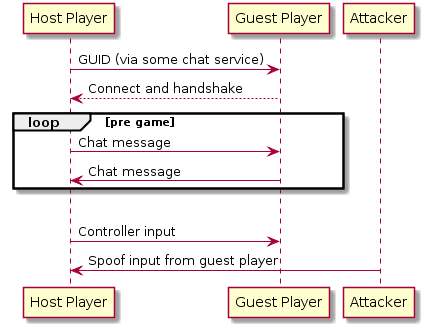
\includegraphics[width=9cm]{Figures/Basic_Sequence}
\end{center}
\vspace{0.3cm}
And the equivalent diagram for the traversal server:
\begin{center}
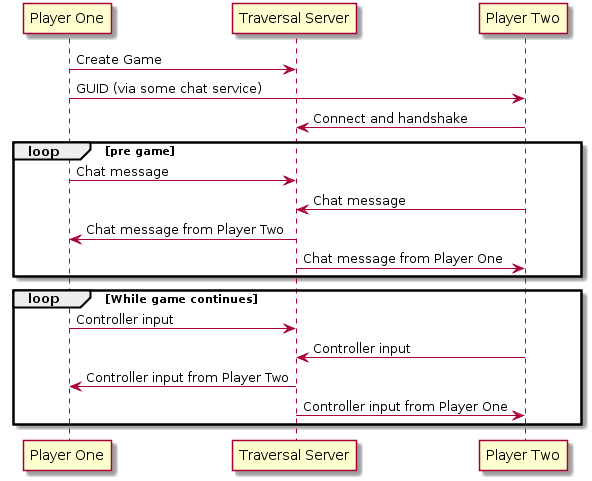
\includegraphics[width=9cm]{Figures/Sequence_Traversal}
\end{center}
\vspace{0.3cm}
\section{Source Code Analysis}
The source code for the Dolphin emulator is available online on github \cite{github-dolphin}. Because of this, we have the opportunity to view the source code to even further interpret the security vulnerabilities.
\section{Traffic Monitoring}
Our first task was to monitor traffic during a game of SSBM via NetPlay. 
The goal of this is to capture and observe network traffic to analyze security vulnerabilities. 
From there we will design and explore possible exploits.
Our experiment here is simple: Play a game of SSBM between two hosts via NetPlay, and monitor the network traffic during the game.

For monitoring, we used the tool "Wireshark" to capture network traffic. During our capture, we used the following filter:

$ ( ip.src == IP_1 \&\& ip.dst == IP_2 ) || (ip.src == IP_2 \&\& ip.dst == IP_1) \&\& udp) $

\vspace{0.3cm}
This filter allowed us to only look at traffic that is to and from the two IP addresses that we used, and only UDP traffic of that.
Initially the traffic was numerous and overwhelming.
We were able to do shorter captures of different stages of the game to narrow down the traffic and more closely associate it with different actions in the game.
For this, we broke the game down into two stages:
\begin{enumerate}  
\item Initial handshake and pre-game
\item During game communication
\end{enumerate}
\vspace{0.5cm}

Some of the initial handshake data is somewhat indecipherable to us. 
However, the pre-game client allows users to "chat" with eachother, and this is easily decipherable. 
An example of such a packet is provided below:
\vspace{0.5cm}

For the actual game communication, it is our analysis that the games send "controller input" back and forth to establish the game. An example of such a packet is provided below:
\vspace{0.5cm}
\begin{center}
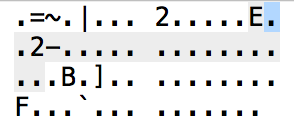
\includegraphics[width=4cm]{Figures/Packet}
\end{center}
\vspace{0.5cm}

Each of these UDP packets contains data about a single controller input.
\section{Experiment 1: Third Party Intervention}
In this first experiment, we explore a fairly simple exploit of the SSBM game via NetPlay.
Our goal, in this experiment, is to interfere with the flow of a game via a third party host.
To achieve this, we use our analysis of the monitored traffic from other games to be able to construct packets that we think will interfere with a game being played by two other hosts. 
\subsection{Packet Spoofing}
To achieve this goal, we will need to be able to construct and send out packets programatically.
Particularly, we will need to construct UDP packets and be able to "spoof" the sender address of such packets.
By this, we mean that we need to be able to indicate that a packet is coming from another host.
We have chosen to implement a simple packet spoofer in Python, and use this to perform the attack.
We use the \textbf{scapy} Python library.
A small sample code snippet is provided below:
\vspace{0.3cm}
\begin{lstlisting}[language=Python]
spoofed_packet = 
   IP(src=src_IP, dst=dst_IP) / 
   UDP(sport=src_port, dport=dst_port) / 
   payload
send(spoofed_packet)
\end{lstlisting}
\vspace{0.3cm}
The \textbf{scapy} library makes the construction and sending of spoofed packets very simple.

\subsection{Attack Overview}
For this experiment, we will first begin a game of SSBM via NetPlay between two hosts.
We will then use a third party computer to spoof packets to interfere with the game.
The third party will spoof packets "pretending" to be one of the hosts (the victim, in this case), and sending facetious and malicious data.
An example sequence diagram for a direct connection is provided below:
\begin{center}
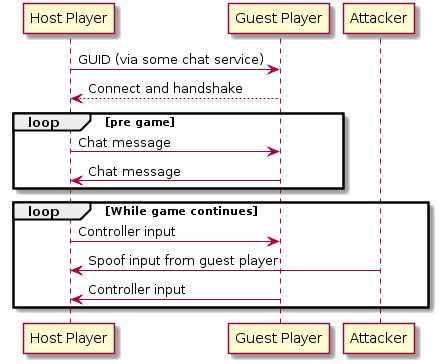
\includegraphics[width=8cm]{Figures/Sequence1}
\end{center}
\vspace{0.5cm}
And the equivalent diagram for a traversal server is:
\begin{center}
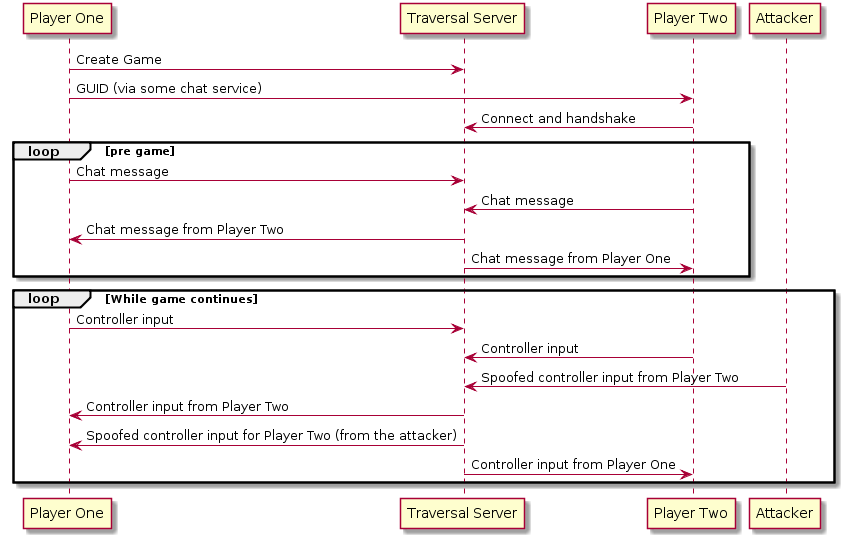
\includegraphics[width=8cm]{Figures/Sequence2}
\end{center}
\vspace{0.5cm}
This experiment is performed on the two types of game connection, namely:
\vspace{0.5cm}
\begin{enumerate}  
\item Direct Connection
\item Traversal Server
\end{enumerate}
\vspace{0.5cm}

The different between the two is that for the direct connection, we will be spoofing packets to the other host. In the case of the traversal server, we will be spoofing messages to the traversal server.


% An example of a floating figure using the graphicx package.
% Note that \label must occur AFTER (or within) \caption.
% For figures, \caption should occur after the \includegraphics.
% Note that IEEEtran v1.7 and later has special internal code that
% is designed to preserve the operation of \label within \caption
% even when the captionsoff option is in effect. However, because
% of issues like this, it may be the safest practice to put all your
% \label just after \caption rather than within \caption{}.
%
% Reminder: the "draftcls" or "draftclsnofoot", not "draft", class
% option should be used if it is desired that the figures are to be
% displayed while in draft mode.
%
%\begin{figure}[!t]
%\centering
%\includegraphics[width=2.5in]{myfigure}
% where an .eps filename suffix will be assumed under latex, 
% and a .pdf suffix will be assumed for pdflatex; or what has been declared
% via \DeclareGraphicsExtensions.
%\caption{Simulation results for the network.}
%\label{fig_sim}
%\end{figure}

% Note that the IEEE typically puts floats only at the top, even when this
% results in a large percentage of a column being occupied by floats.


% An example of a double column floating figure using two subfigures.
% (The subfig.sty package must be loaded for this to work.)
% The subfigure \label commands are set within each subfloat command,
% and the \label for the overall figure must come after \caption.
% \hfil is used as a separator to get equal spacing.
% Watch out that the combined width of all the subfigures on a 
% line do not exceed the text width or a line break will occur.
%
%\begin{figure*}[!t]
%\centering
%\subfloat[Case I]{\includegraphics[width=2.5in]{box}%
%\label{fig_first_case}}
%\hfil
%\subfloat[Case II]{\includegraphics[width=2.5in]{box}%
%\label{fig_second_case}}
%\caption{Simulation results for the network.}
%\label{fig_sim}
%\end{figure*}
%
% Note that often IEEE papers with subfigures do not employ subfigure
% captions (using the optional argument to \subfloat[]), but instead will
% reference/describe all of them (a), (b), etc., within the main caption.
% Be aware that for subfig.sty to generate the (a), (b), etc., subfigure
% labels, the optional argument to \subfloat must be present. If a
% subcaption is not desired, just leave its contents blank,
% e.g., \subfloat[].


% An example of a floating table. Note that, for IEEE style tables, the
% \caption command should come BEFORE the table and, given that table
% captions serve much like titles, are usually capitalized except for words
% such as a, an, and, as, at, but, by, for, in, nor, of, on, or, the, to
% and up, which are usually not capitalized unless they are the first or
% last word of the caption. Table text will default to \footnotesize as
% the IEEE normally uses this smaller font for tables.
% The \label must come after \caption as always.
%
%\begin{table}[!t]
%% increase table row spacing, adjust to taste
%\renewcommand{\arraystretch}{1.3}
% if using array.sty, it might be a good idea to tweak the value of
% \extrarowheight as needed to properly center the text within the cells
%\caption{An Example of a Table}
%\label{table_example}
%\centering
%% Some packages, such as MDW tools, offer better commands for making tables
%% than the plain LaTeX2e tabular which is used here.
%\begin{tabular}{|c||c|}
%\hline
%One & Two\\
%\hline
%Three & Four\\
%\hline
%\end{tabular}
%\end{table}


% Note that the IEEE does not put floats in the very first column
% - or typically anywhere on the first page for that matter. Also,
% in-text middle ("here") positioning is typically not used, but it
% is allowed and encouraged for Computer Society conferences (but
% not Computer Society journals). Most IEEE journals/conferences use
% top floats exclusively. 
% Note that, LaTeX2e, unlike IEEE journals/conferences, places
% footnotes above bottom floats. This can be corrected via the
% \fnbelowfloat command of the stfloats package.


% conference papers do not normally have an appendix


% use section* for acknowledgment
%\section*{Acknowledgment}
%
%
%The authors would like to thank...





% trigger a \newpage just before the given reference
% number - used to balance the columns on the last page
% adjust value as needed - may need to be readjusted if
% the document is modified later
%\IEEEtriggeratref{8}
% The "triggered" command can be changed if desired:
%\IEEEtriggercmd{\enlargethispage{-5in}}

% references section

% can use a bibliography generated by BibTeX as a .bbl file
% BibTeX documentation can be easily obtained at:
% http://mirror.ctan.org/biblio/bibtex/contrib/doc/
% The IEEEtran BibTeX style support page is at:
% http://www.michaelshell.org/tex/ieeetran/bibtex/
\bibliographystyle{IEEEtran}
% argument is your BibTeX string definitions and bibliography database(s)
\bibliography{bib}
%
% <OR> manually copy in the resultant .bbl file
% set second argument of \begin to the number of references
% (used to reserve space for the reference number labels box)
%\begin{thebibliography}{1}
%
%\bibitem{IEEEhowto:kopka}
%H.~Kopka and P.~W. Daly, \emph{A Guide to \LaTeX}, 3rd~ed.\hskip 1em plus
%  0.5em minus 0.4em\relax Harlow, England: Addison-Wesley, 1999.
%
%\end{thebibliography}




% that's all folks
\end{document}


